\renewcommand{\BrainFuckChapter}{%
  {+}{+}{[}{-}{-}{-}{-}{-}{-}{-}{-}{-}{-}{>}{+}{<}{]}{>}{.}{-}{-}{-}{-}{-}{.}{+}{+}{+}{+}{+}{+}{+}{+}{+}{+}{+}{.}{>}{-}{[}{-}{-}{-}{-}{-}{>}{+}{<}{]}{>}{-}{.}{-}{-}{[}{-}{-}{-}{>}{+}{+}{<}{]}{>}{.}{-}{-}{[}{-}{-}
  {>}{+}{+}{+}{<}{]}{>}{.}{[}{-}{-}{-}{>}{+}{+}{<}{]}{>}{+}{+}{.}{[}{-}{-}{>}{+}{+}{+}{+}{+}{<}{]}{>}{-}{.}{+}{[}{-}{-}{-}{>}{+}{<}{]}{>}{.}{+}{+}{+}{+}{.}{-}{-}{-}{-}{-}{-}{-}{-}{-}{-}{-}{.}{+}{+}{+}{+}{.}{-}{-}
  {-}{-}{.}{-}{[}{-}{-}{-}{>}{+}{<}{]}{>}{+}{+}{.}{[}{-}{>}{+}{+}{+}{+}{+}{<}{]}{>}{-}{.}{-}{-}{[}{-}{-}{-}{>}{+}{<}{]}{>}{-}{.}{-}{-}{-}{-}{-}{-}{-}{-}{-}{-}{-}{.}{+}{+}{+}{+}{+}{+}{.}{-}{.}{+}{+}{+}{+}{+}{.}{-}
  {-}{-}{-}{<}{-}{>}{-}{<}{>}{<}{+}{<}{+}{<}{+}{-}{>}{-}{+}{<}{<}{+}{+}{<}{-}{<}{>}{-}{-}{-}{<}{>}{+}{>}{>}{<}{<}{+}{<}{>}{-}{<}{<}{+}{<}{>}{<}{<}{+}{-}{+}{-}{<}{+}{<}{+}{>}{<}{+}{<}{>}{<}{>}{+}{-}{+}{-}{+}{>}{-}
}

\renewcommand{\LifeChapter}{y}
\chapter{\mhsII{} -- Optimizations}

\label{sec:mhs2o}
In this chapter we present the sequential version our novel \ac{MHS}
generation algorithm, dubbed \ac{MHSII}.
%
As explained in
\CrefPageParen{sec:intro:research-goals:algorithmic-efficiency}, our
goal in this chapter is to improve the computational efficiency of the
\staccato{} algorithm.

This chapter is divided as follows.
%
First, we introduce our \ac{MHS} generation algorithm.
%
Second, we provide a formal analysis of the proposed algorithm.
%
Third, we discuss the data-structures used in the algorithm's
implementation.
%
Fourth, we discuss some practical aspects of the algorithm's
utilization.
%
Fifth and lastly, we evaluate the performance of our algorithm.

\section{Approach}
\label{sec:mhs2o:approach}
%
The proposed algorithm consists of an improved version of the
\staccato{} algorithm \citep{Abreu09b}
(\CrefPageSee{alg:intro:staccato}).
%
In contrast to the original algorithm, we propose $3$ optimizations
that prevent redundant calculations (\Cref{fig:mhs2o:intuition}).

\begin{algorithm}
  \begin{description}
  \item[Inputs:]\ $(U, S, d=\emptyset, D=\emptyset)$
  \item[Output:]\ Minimal hitting set collection $D$
  \end{description}

  \begin{algorithmic}[1]
    \CIF{$\exists_{s \in S} : s \cap U = \emptyset$} \algorithmiccomment{\Opt{3}} \label{alg:mhs2o:opt3.1}
    \CSTATE \Return $D$ \label{alg:mhs2o:opt3.2}
    \EndIf
    \If{$S \not= \emptyset$} \label{alg:mhs2o:divide}
    \CSTATE $U \gets U \setminus \set{j \mid j \in U \wedge (\nexists_{s \in S}: j\in s)}$\algorithmiccomment{\Opt{2}}  \label{alg:mhs2o:opt2}
    \For{$j \in  \fn{Rank}(U, S)$} \label{alg:mhs2o:rank}
    \State $S^\prime \gets \set{s \mid s \in S \wedge j \in s}$ \label{alg:mhs2o:S'}
    \CSTATE $U \gets U \setminus \set{j}$   \algorithmiccomment{\Opt{1}} \label{alg:mhs2o:opt1}
    \State $D \gets \fn{MHS^\text{\smaller2}}(U, S \setminus S^\prime, d \cup \set{j}, D)$
    \EndFor
    \Else
    \If{$\nexists_{d^\prime\in D}: d^\prime\subseteq d$} \label{alg:mhs2o:isminimal}
    \State $D \gets D \setminus \set{d^\prime \mid d^\prime \in D \wedge  d \subseteq d^\prime}$ \label{alg:mhs2o:purge}
    \State $D \gets D \cup \set{d}$ \label{alg:mhs2o:addD}
    \EndIf
    \EndIf
    \State \Return $D$
  \end{algorithmic}
  \caption{\acs{MHSII} -- Optimizations}
  \label{alg:mhs2o}
\end{algorithm}

\begin{figure}[!ht]
  \captionsetup[subfigure]{aboveskip=1em,belowskip=1em}  \begin{subfigure}[b]{\columnwidth}
    \includegraphics[page=8]{figures/mhs2/figures/opts/main}
    \caption{Optimization 1\label{fig:mhs2o:opt1-intuition}}
  \end{subfigure}

  \begin{subfigure}[b]{\columnwidth}
    \includegraphics[scale=1.1,page=9]{figures/mhs2/figures/opts/main}
    \caption{Optimization 2\label{fig:mhs2o:opt2-intuition}}
  \end{subfigure}

  \begin{subfigure}[b]{\columnwidth}
    \includegraphics[scale=1.1,page=10]{figures/mhs2/figures/opts/main}
    \caption{Optimization 3\label{fig:mhs2o:opt3-intuition}}
  \end{subfigure}
  \caption{Optimizations' visual intuition\label{fig:mhs2o:intuition}}
\end{figure}

The first optimization (line \ref{alg:mhs2o:opt1} and
\Cref{fig:mhs2o:opt1-intuition}) prevents multiple evaluations of the
same set, as it was the case of $\set{2,3}$ in the example presented
in \CrefPageParen{fig:intro:staccato-search-tree}.
%
Removing element $j$ from $U$ (and, consequently, from $S$) after its
evaluation has the practical effect of reducing the search space to a
spanning tree of the original search tree.

To see the effect of this optimization, consider the example in
\Cref{fig:mhs2o:opt1-intuition}.
%
The example depicts the largest search trees for $U=\set{1,2,3}$ with
and without optimization $1$.
%
Each box represents a call to algorithm and the value contained inside
each box represents the value of $d$ for that particular call.

Without the proposed optimization, a large amount of redundant work
would be performed (\eg, $8$ evaluations of the set $\set{1,2,3}$).
%
With the proposed optimization, it is guaranteed that every set is
evaluated at most once.
%
Concretely, the upper-bound size of the search space without
optimizations can be described with the following
expression:
\begin{equation}
  \fn{a}(U) = 1 + \fn{b}(|U|)
  \label{eq:mhs2o:no-opt-upper-bound}
\end{equation}
\begin{equation}
  \fn{b}(x) = \begin{cases}
    x + x * \fn{b}(x-1) & \textrm{if~} x > 0 \\
    0              & \textrm{otherwise}
  \end{cases}
\end{equation}
\noindent
$\fn{b}(x)$ is described on the On-Line Encyclopedia of Integer
Sequences as the number of permutations of nonempty subsets of a set
with size $x$. Since the empty set may also be a solution for a given
problem, it is necessary to add $1$ to the result of $\fn{b}(x)$ (see
\url{https://oeis.org/A007526} for further information).

On the other hand, the upper-bound size of the search space for the
optimized algorithm is given by the following expression:
\begin{equation}
  \label{eq:mhs2o:opt-upper-bound}
  \displaystyle \fn{c}(U) = 2^{|U|}
\end{equation}
\noindent
To illustrate both upper-bound search space sizes, both functions are
plotted in \Cref{fig:mhs2o:search-space-comparison}.
%
We can clearly see that $\fn{a}(U)$ grows much faster than $\fn{c}(U)$
(note the log scale).

\begin{figure}[!ht]
  \includegraphics[width=0.8\columnwidth,page=3]{figures/mhs2/figures/opts/main}
  \caption{Search space size comparison\label{fig:mhs2o:search-space-comparison}}
\end{figure}

The second optimization (line \ref{alg:mhs2o:opt2} and
\Cref{fig:mhs2o:opt2-intuition}) preemptively filters elements of $U$
not contained in any set in $S$.
%
As this filtering process reduces the size of $U$ and, consequently,
the size of the data structures holding $(U,S)$, the operations
performed on $(U,S)$, such as the ranking calculation, become
faster.

The third optimization (lines \ref{alg:mhs2o:opt3.1},
\ref{alg:mhs2o:opt3.2}, and \Cref{fig:mhs2o:opt3-intuition}) prevents
the examination of branches such that $\exists_{s \in S} : s \cap U =
\emptyset$, \ie, there is at least one set that cannot be hit by any
element in $U$.
%
The existence of such a set in $S$
guarantees, by definition, that no \ac{HS} will be found
(\CrefPageSee{cor:intro:unsatisfiablity}).

\section{Algorithm Analysis}
\label{sec:mhs2o:analysis}
In this section we discuss the algorithm from a more formal point-of-view.
%
First, we prove the algorithm's soundness and completeness.%
\footnote{In this context, and assuming no cutoffs are enforced, the
  algorithm is sound if all computed sets are \acp{MHS}.
  %
  A complete algorithm should compute all \acp{MHS}.
  %
  It is worth noting that a sound algorithm may miss some \acp{MHS}
  and a complete algorithm may compute some sets that are not
  \acp{MHS} (\ie, soundness~$\nLeftrightarrow$~completeness).  }
%
Second, we provide some intuition on the complexity of the different
operations performed by the \ac{MHSII} algorithm.

\subsection{Completeness/Soundness analysis}
\label{sec:mhs2o:analysis:soundcomplete}
\begin{lemma}
  All sets computed by \ac{MHSII} are \acp{HS}.
\end{lemma}
\begin{proof}
  Suppose \ac{MHSII} is set to compute a single \ac{HS}.
  %
  At each step, an element $j \in U$ is selected and \ac{MHSII} is
  recursively called for $S \setminus S^\prime$ with set $d \cup \set{j}$.
  %
  This procedure is repeated until $S = \emptyset$, at which point
  $\emptyset$ is a \ac{HS} for $S$ (\CrefPageSee{cor:intro:emptyHS}).

  Let $S^\prime_n$ and $j_n$ be the $S^\prime$ set and $j$ element at the $n^{th}$
  recursive level.  Since $\forall_{s \in S_n^\prime} : j_n \in s$ (\ie,
  $\set{j_n}$ is a hitting set for $S_n^\prime$), it follows that:
  \begin{equation}
    \bigwedge_1^n  \HS(U_n,S^\prime_n,d_n)
  \end{equation}

  From \CrefPageParen{cor:intro:associativity}, as
  $S = \bigcup_1^n S_n^\prime$ and $d = \bigcup_1^n d_n$, it follows that:
  \begin{equation}
    \bigwedge_1^n  \HS(U_n,S^\prime_n,d_n) \implies \HS(U, S, d)
  \end{equation}
\end{proof}

\begin{lemma}[Completeness]
  \label{lem:mhs2o:completeness}
  \staccato{} computes all \acp{MHS} for a problem $(U,S)$.
\end{lemma}
\begin{proof}
  Suppose \staccato{} does not stop the branch exploration after a
  \ac{HS} is found.
  %
  Under this constraint, it follows that the algorithm comprehensively
  explores every element in $\powSet{U}$, which contains all
  \acp{HS} for $(U,S)$ and, consequently, all \acp{MHS} for $(U,S)$.

  By stopping the branch exploration after an \ac{HS} $d$
  is found, the \acp{HS} contained in
  $\set{d \cup d^\prime \mid d^\prime \subseteq (U\setminus d) \wedge
    d^\prime \not= \emptyset}$ are ignored.
  %
  Since, by definition $\HS(U,S,d) \wedge (d^\prime \not= \emptyset)
  \implies \neg\MHS(U,S,d \cup d^\prime)$, we can conclude that even
  though some \acp{HS} are ignored, all \acp{MHS} are nonetheless
  computed.
\end{proof}

\begin{theorem}
  Optimization $1$ preserves completeness.
\end{theorem}
\begin{proof}
  Let $ \Omega = \powSet{U \setminus (d \cup \set{j})}$.
  %
  After every recursive call to \staccato{}, it is guaranteed that all
  \acp{MHS} contained in $K = \set{d \cup \set{j} \cup e \mid e \in
    \Omega}$ are evaluated (\Cref{lem:mhs2o:completeness}).

  By removing $j$ from $U$ for subsequent calls of \staccato{} under
  the same search tree branch, the algorithm prevents subsequent
  evaluations of the sets contained in $K$, only calculating the
  \acp{MHS} contained in $L = \set{d \cup e \mid e \in \Omega}$.
  %
  Since $K \cup L = \set{d \cup{} e \mid e \in \powSet{U \setminus d}}$,
  the optimization preserves completeness.
\end{proof}

\begin{theorem}
  Optimization $2$ preserves completeness.
\end{theorem}
\begin{proof}
  Let $K = \set{j \mid j \in U \wedge (\nexists_{s \in S}: j\in s)}$.
  By definition, it follows that:
  \begin{equation}
    \HS(U,S, d) \wedge d \cap K \not=\emptyset \implies \neg \MHS(U,S, d)
  \end{equation}
  Since removing elements in $K$ from $U$ only prevents the
  calculation of sets that are guaranteed not to be \acp{MHS}, we can
  conclude that the optimization preserves completeness.
\end{proof}

\begin{theorem}
  Optimization $3$ preserves completeness.
\end{theorem}
\begin{proof}
  From \CrefPageParen{cor:intro:unsatisfiablity}, it follows that:
  \begin{equation}
    \exists_{s \in S} : s \cap U = \emptyset \implies \nexists_{d} : \HS(U,S,d)
  \end{equation}

  Since halting the exploration of a branch whenever the
  aforementioned condition holds only prevents the examination of sets
  that are guaranteed not to be \acp{HS}, we can conclude that the
  optimization preserves completeness.
\end{proof}

\begin{corollary}
  \ac{MHSII} is complete.
\end{corollary}

\begin{theorem}[Soundness]
  If all \acp{MHS} are evaluated, all sets computed by \ac{MHSII} are \acp{MHS}.
\end{theorem}

\begin{proof}
  Given the fact that a set $d$ is only added to $D$ if and only if
  $\nexists_{d^\prime\in D}: d^\prime\subseteq d$ and, prior to its
  addition, all sets in $\set{d^\prime \mid d^\prime \in D \wedge d
    \subseteq d^\prime}$ are removed from $D$, it follows that, at any
  given point, the sets in $D$ are relatively minimal (\ie,
  $\nexists_{d,d^\prime\in D}: d^\prime\subset d$).
  %
  Since, by hypothesis, all existent \acp{MHS} for the problem are
  evaluated (and therefore added to $D$) and all sets contained in $D$
  are always relatively minimal, no absolutely non-minimal \ac{HS} is
  contained in $D$.
\end{proof}

\subsection{Complexity Analysis}
\label{sec:mhs2o:analysis:complexity}
As shown in \citep{Garey90}, the \ac{MHS} problem is NP-Hard.
%
In this section we provide upper-bound values for the complexity of
the operations performed in each call of \ac{MHSII}.

Each time \ac{MHSII} is called it:
\begin{enumerate}
\item Checks whether the current sub-problem has any solutions:
  $\bigO{M\times N}$, where $M = |U|$ and $N = |S|$ (line
  \ref{alg:mhs2o:opt3.1}, optimization 3).
\item Checks whether the current sub-problem is trivially solvable:
  $\bigO{1}$ (line \ref{alg:mhs2o:divide}).
\end{enumerate}

If the problem is not trivially solvable, the algorithm:
\begin{enumerate}
\item Removes elements from $U$ that are guaranteed not to form
  \acp{MHS}: $\bigO{M\times N}$ (line \ref{alg:mhs2o:opt2},
  optimization 2).
\item Generates heuristic values for each element in $U$: at least
  $\bigO{M}$, usually $\bigO{M\times N}$ (line \ref{alg:mhs2o:rank}).
\item Ranks elements of $U$ according to their heuristic values:
  $\bigO{M \times \log(M)}$ (line \ref{alg:mhs2o:rank}).
\item Prepares, for each element of the ranking, a sub-problem to be
  solved: $\bigO{M^2 \times N}$ (lines \ref{alg:mhs2o:S'} --
  \ref{alg:mhs2o:opt1}).
  \begin{enumerate}
  \item Simplifies the problem: $\bigO{M\times N}$ (line
    \ref{alg:mhs2o:S'}).
  \item Removes the current element from $U$: $\bigO{1}$ (line
    \ref{alg:mhs2o:opt1}, optimization 1).
  \end{enumerate}
\end{enumerate}

If the problem is trivially solvable, the algorithm:
\begin{enumerate}
\item Checks if the current set $d$ is minimal with respect to $D$:
  $\bigO{I\times K\times L}$, where $I = |d|, K = |D|, $ and $L =
  \sum_{d^\prime\in D} \frac{|d^\prime|}{K}$ (line
  \ref{alg:mhs2o:isminimal}).
\item Removes non-minimal \acp{HS} from $D$: $\bigO{I\times K\times
    L}$ (line \ref{alg:mhs2o:purge}).
\item Adds $d$ to $D$: $\bigO{I}$ (line \ref{alg:mhs2o:addD}).
\end{enumerate}

\section{Data structures}
\label{sec:mhs2o:datastructures}
To have an efficient implementation of \ac{MHSII} the following
operations must be performed efficiently:
\begin{enumerate}
\item Remove elements from $S$ (line \ref{alg:mhs2o:S'});
\item Check set for relative minimality (line \ref{alg:mhs2o:isminimal});
\item Purge proper super sets of a set from collection $D$ (line
  \ref{alg:mhs2o:purge});
\end{enumerate}

In the remainder of this section, we analyze the data structures used
in our reference implementation.
%
The implementation is available at \mhsIIURL{}.

\subsection{Encoding \texorpdfstring{$(U,S)$}{(U,S)}}
To efficiently encode and manipulate $(U,S)$, we make use of a $N
\times M$ binary matrix (referred to as $A$) where each of the
matrix's rows encodes the membership of each element $j \in U$ in a
particular set $S_i$ (\ie, $A_{ij} = [j \in S_i]$, where $[.]$ denotes
Iverson's operator: $[\mTrue] = 1, [\mFalse] = 0$).

To avoid making multiple copies of the matrix when a modification to
$(U,S)$ is required, we make use of a data structure we refer to as a
\emph{filter}.
%
In practice, a filter is a vector storing which columns/rows should be
ignored at each stage of the algorithm's execution.
%
Consequently, the resultant data structure is a 3-tuple $(A,fc,fr)$
representing the original $(U,S)$ matrix, and the filtered
columns/rows respectively.

\begin{figure}[!ht]
  \includegraphics[page=4]{figures/mhs2/figures/opts/main}
  \caption{Example search tree showing binary matrix for $(U,S)$ (no
    optimizations)}
  \label{fig:mhs2o:search-tree-spectrum}
\end{figure}
To illustrate how this works in practice, consider the example in
\Cref{fig:mhs2o:search-tree-spectrum} showing the matrix
representation of $(U,S)$.
%
Similarly to \CrefPageParen{fig:intro:staccato-search-tree}, each node
in the search tree represents a call to the function (all the
parameters as well as the return value are encoded as a table).
%
Colored matrix cells represent the filtered elements of the original
matrix.
%
Each circle marks the element that triggered the filtering of
corresponding row.

A na\"{i}ve implementation of such filters could be done with Boolean
vectors where each cell encodes the state of each column/row.
%
Even though this approach is more efficient than copying the matrix
multiple times, it is possible to improve this structure to be more
efficient when iterating over a filtered matrix.

To that end, we use an integer vector where each cell contains the
index of the next unfiltered element.
%
Such filter vectors have $n+1$ elements, where $n$ is the maximum
number of elements to be filtered.
%
The filter vector indexes are zero-based so it is possible to
filter the first row/column of the matrix, which are one-based.
%
The initial state for $n$
element filter is formally defined as $f_i=(i+1)\mod{(n + 1)}$.

To iterate using one of such filters, a counter starting at $0$ must
be kept and, after each iteration, it is updated as $i=f_i$.
%
The loop ends when the counter returns its value to $0$.

To filter an element $i$, one must iterate back from $j=i-1$ until
$f_j\not=i$, setting each $f_j$ to be equal to $f_i$.
%
In contrast to the na\"{i}ve approach, when all elements are filtered,
the loop is never executed, improving the efficiency.
%

\Cref{fig:mhs2o:filter-example} depicts the states of a filter for a
maximum of four elements after filtering elements $3$, $1$, $2$, and,
finally, $4$.
\begin{figure}[!ht]
  \begin{tabular}[ht]{c|nnnnn}
    $i$                & \cclre $0$ & \cclra $1$           & \cclrb $2$           & \cclrc $3$           & \cclrd $4$           \\
    \hline
    Initial state      & \cclra $1$ & \cclrb $2$           & \cclrc $3$           & \cclrd $4$           & \cclre $0$           \\
    After filter $i=2$ & \cclra $1$ & \cclrc $3$           & \cclrc \circled{$3$} & \cclrd $4$           & \cclre $0$           \\
    After filter $i=4$ & \cclra $1$ & \cclrc $3$           & \cclrc $3$           & \cclre $0$           & \cclre \circled{$0$} \\
    After filter $i=1$ & \cclrc $3$ & \cclrc \circled{$3$} & \cclrc $3$           & \cclre $0$           & \cclre $0$           \\
    After filter $i=3$ & \cclre $0$ & \cclre $0$           & \cclre $0$           & \cclre \circled{$0$} & \cclre $0$           \\
  \end{tabular}
  \caption{Filter with $4$ elements}
  \label{fig:mhs2o:filter-example}
\end{figure}



\subsection{Encoding \texorpdfstring{$D$}{D}}
\label{sec:mhs2o:trie}
To efficiently store \acp{HS}, check their relative minimality and
purge non-\acp{MHS}, we use the trie data structure.
%
A trie is a tree-like data structure where the set of node values in
the path from the root to a marked node corresponds to an element (in
this case a \ac{HS}) stored in the trie.

To operate a trie, we assume the existence of the following basic
operations:
\begin{itemize}
\item $\fn{isMarked}(n)$: Checks whether node $n$ is marked. If node
  $n$ is an invalid node (denoted as $\times$) the function returns
  $\mFalse$.
\item $\fn{getChild}(n,e)$: Returns the child node of $n$ with value
  $e$ or $\times$ if no child of node $n$ has value $e$.
\item $\fn{getChildren}(n)$: Returns the node values of the children
  of node $n$.
\item $\fn{setChild}(n,e,n^\prime)$: Assigns node $n^\prime$ as the
  child of $n$ with value $e$. If $n^\prime = \times$, the function
  removes the child node with value $e$ instead.
\end{itemize}


%
An important prerequisite to efficiently implement the required
(complex) trie operations is that the elements in all \acp{HS} are
ordered (in the following we assume ascending order).
%
On the one hand, the ordering assumption guarantees that any \ac{HS}
has a unique representation (\eg, \set{1,2,3} \vs{} \set{2,3,1} or
\set{3,2,1}).
%
On the other hand, it guarantees that the trie itself has an ordered
structure (\ie, $\nexists_{n,n^\prime,e,e^\prime} : n^\prime =
\fn{getChild}(n,e) \wedge e^\prime \in \fn{getChildren}(n^\prime)
\wedge e^\prime \leq e $), enabling a reduction in the amount of nodes
to be processed when checking for minimality and purging super sets.

\begin{figure}[!ht]
  \begin{subfigure}[b]{0.5\columnwidth}
    \centering
    \includegraphics[page=6]{figures/mhs2/figures/opts/main}
    \caption{Using unordered sets\label{fig:mhs2o:trieunordered}}
  \end{subfigure}%
  %
  \begin{subfigure}[b]{0.5\columnwidth}
    \centering
    \includegraphics[page=5]{figures/mhs2/figures/opts/main}
    \caption{Using ordered sets\label{fig:mhs2o:trieordered}}
  \end{subfigure}%
  %
  \caption{A trie encoding $6$ \acsp{HS}\label{fig:mhs2o:trie}}
\end{figure}

As an example consider two possible tries storing \acp{HS}
$\set{1,2,3,5}$, $\set{1,2,4,6}$, $\set{1,2,5}$, $\set{2,4,6}$,
$\set{2,4,6,7,8}$, and $\set{8}$, which are presented in
\Cref{fig:mhs2o:trie}.
%



\begin{algorithm}[ht]
  \begin{description}
  \item[Inputs:]\ $(n, d)$
  \item[Output:]\ Boolean
  \end{description}
  \begin{algorithmic}[1]
    \If{$\fn{isMarked}(n)$}
    \State \Return $\mFalse$
    \ElsIf{$n \not= \times$}
    \While{$d \not= \emptyset$}
    \State $e \gets \fn{min}(d)$
    \State $d \gets d \setminus \set{e}$
    \State $n^\prime \gets \fn{getChild}(n, e)$
    \If{$\neg \fn{isMinimal}(n^\prime, d)$}
    \State \Return $\mFalse$
    \EndIf
    \EndWhile
    \EndIf
    \State \Return $\mTrue$

  \end{algorithmic}
  \caption{$\fn{isMinimal}$}
  \label{alg:mhs2o:isminimal-impl}
\end{algorithm}

The algorithm for checking the minimality of an \ac{HS} in view of the
\acp{HS} encoded in the trie (line \ref{alg:mhs2o:isminimal} in
\Cref{alg:mhs2o}) is presented in \Cref{alg:mhs2o:isminimal-impl}.
%
The algorithm attempts to find a path from the root node to a marked
node composed exclusively of elements from set $d$.
%
If no such path is found, set $d$ has no subsets in the trie and,
consequently, is minimal.
%
In practice, the algorithm works by iteratively selecting an element
$e$ from $d$ and recursively exploring the child node with value $e$
using the set $d\setminus\set{e}$.
%
Since the trie has an ordered structure, the elements of $d$ are
orderly selected and removed from $d$, avoiding the need to explore
different permutations of the same sets.

\begin{algorithm}[ht]
  \begin{description}
  \item[Inputs:]\ $(n, d)$
  \item[Output:]\ Node
  \end{description}

  \begin{algorithmic}[1]
    \If{$d = \emptyset$}
    \State \Return $\times$
    \Else
    \State $e \gets \fn{min}(d)$
    \For{$e^\prime : e^\prime \in \fn{getChildren}(n) \wedge e^\prime \leq e$}
    \State $d^\prime \gets d$
    \If{$e^\prime = e$}
    \State $d^\prime \gets d^\prime \setminus  \set{e}$
    \EndIf
    \State $n^\prime \gets \fn{purgeSuperSets}(\fn{getChild}(n, e^\prime),d^\prime)$
    \State $n \gets \fn{setChild}(n, e^\prime, n^\prime)$
    \EndFor
    \EndIf
    \If{$\neg \fn{marked}(n) \wedge \fn{getChildren}(n) = \emptyset$}
    \State \Return $\times$
    \EndIf
    \State \Return $n$
  \end{algorithmic}
  \caption{$\fn{purgeSuperSets}$}
  \label{alg:mhs2o:purgesupersets}
\end{algorithm}

The algorithm for purging all supersets of a particular \ac{HS} from
the trie (line \ref{alg:mhs2o:purge} in
\Cref{alg:mhs2o}) is presented in
\Cref{alg:mhs2o:purgesupersets}.
%
The algorithm attempts to find all the paths from the root node to
some node in the trie containing all elements from set $d$ and removes
them.
%
In practice, the algorithm explores the tree recursively and, whenever
the value ($e$) of the node being inspected is contained in $d$, $e$
is removed from $d$ for subsequent recursive calls in that particular
branch.
%
Whenever $d$ becomes empty (signaling that all elements in the
original set $d$ are contained in the path to node $n$), that
particular subtree is removed from the trie.

While removing the subtree when $d$ is empty effectively removes all
supersets from the trie, it may also leave extraneous nodes in the
trie (\ie, nodes that are not marked and do not have marked nodes in
their sub-trees).
%
To remove such extraneous nodes, after exploring the sub-trees of a
particular node, the algorithm checks if it is marked and, if not, if
it has no children.
%
If the node is not marked and has no children, it is also removed from
the trie.

\section{Practical Considerations}
In this section we discuss domain-specific aspects of the proposed
algorithm.
%
First, we discuss the selection of the heuristic as a way of improving
the performance of \ac{MHSII} in a particular domain.
%
Second, we present two pre-processing operations aimed at decreasing
the problem's complexity while guaranteeing that the solution remains
unaltered.

\subsection{Heuristics}
\label{sec:mhs2o:heuristics}
To fine tune the algorithm for a domain specific goal, the algorithm
uses the concept of heuristic to drive the search by determining the
shape and order of exploration of the search tree.
%
An example of heuristic would be to rank the elements of $U$ according
to the number of sets they hit.
%
Concretely, such a heuristic would be defined as follows:
\begin{equation}
  \fn{\mathcal H}(j) = \big|\set{s \mid s \in S \wedge j \in s}\big|
\end{equation}
%
Intuitively, this heuristic attempts to greedily minimize the size of
the computed \acp{HS}.

In the context of \ac{SFL}, as faults may not be consistently
triggered, failing transactions convey information on the possible
causes of a system malfunction whereas successful transactions help
the diagnosis system to exonerate components that would otherwise be
inaccurately judged as faulty.
%
As the goal of diagnosis is to find the best explanation for an error,
using a heuristic that minimizes the size of the computed \acp{HS}
may not be ideal.

To convey this intuition to \staccato{}, the \textit{Ochiai}
similarity coefficient \citep{Meyer04} was used as a heuristic
\citep{Abreu09b}.
%
The selection of this particular similarity coefficient was based on
the results of previous work on similarity-based \ac{SFL} showing
evidence that, for real-world diagnostic scenarios, \textit{Ochiai}
provides good heuristic results \citep{Abreu07}.
%
Concretely, the heuristic is defined as follows:
\begin{equation}
  \fn{\mathcal H}(j) = \frac{n_{11}(j)}{\sqrt{\big(n_{11}(j)+n_{01}(j)\big)*\big(n_{11}(j)+n_{10}(j)\big)}}
\end{equation}
where
\begin{itemize}
\item $n_{11}$: Number of failing transactions where $j$ was active.
\item $n_{10}$: Number of failing transactions where $j$ was not
  active.
\item $n_{01}$: Number of passing transactions where $j$ was active.
\end{itemize}

\begin{figure}[!ht]
  \includegraphics[page=7]{figures/mhs2/figures/opts/main}
  \caption{Example search tree with heuristic values (with
    optimizations)}
  \label{fig:mhs2o:heuristic:search-tree}
\end{figure}

To illustrate how the heuristic works in practice, consider the search
tree in \Cref{fig:mhs2o:heuristic:search-tree} in which the heuristic
values are presented.
%
Similarly to \CrefPageParen{fig:mhs2o:search-tree-spectrum}, each node
in the search tree represents a call to the function.
%
Unlike \Cref{fig:mhs2o:search-tree-spectrum}, instead of only
representing the conflicts, the full hit spectrum is
presented\footnote{Recall that every node having all rows with
  $e_i = 1$ (\ie, the conflicts) filtered represents a (potentially
  non-minimal) diagnostic candidate.}.
%
Also, \Cref{fig:mhs2o:heuristic:search-tree} depicts a search tree
for the fully optimized \ac{MHS} algorithm.
%

We can see that the ranking for the outermost call the component
evaluation order is $\angledlist{c_2,c_1,c_4,c_3}$.
%
Intuitively, this is due to the fact that $c_1$ and $c_2$ share the
same activation pattern in failing transactions but $c_1$ was also
activated in a passing transaction whereas $c_2$ was not.
%
The same logic can be applied between $c3$ and $c_4$.
%
Since $c_1$ and $c_2$ were activated in more failing transactions than
$c_3$ and $c_4$, they are evaluated first.


It is important to note that, due to the fact that the failing
transactions get filtered during the algorithm's execution, the value
of the heuristic for a particular element may vary for different nodes
in the search tree.



\subsection{Ambiguity Group Removal}
\label{sec:mhs2o:ambiguity-groups}
Ambiguity groups \citep{Sanchez11b} occur when two or more elements of
$U$ are members of the same sets in $S$ (\ie, for two elements
$j_1,j_2$, $\forall_{s\in S}: j_1 \in s \Leftrightarrow j_2 \in s$).
%
If such groups exist, if follows that:
\begin{equation}
  \MHS(U,S,d \cup \set{j_1}) \Leftrightarrow \MHS(U,S,d \cup \set{j_2})
\end{equation}
%
Intuitively, the above formula states that the elements from an
ambiguity group are interchangeable since they hit the same sets.
%
It is possible to take advantage of this fact by collapsing the
different ambiguity groups into single elements (and making sure
such information is available), thus reducing the search space.
%

As an example consider the following \ac{MHS} problem:
\begin{equation}
  \begin{array}{l}
    U = \set{1,2,3,4}\\
    S = \set{\set{1,2}, \set{3,4}}\\
    D = \set{\set{1,3}, \set{1,4}, \set{2,3},\set{2,4}}
  \end{array}
\end{equation}
%
For this example elements $1$ and $2$ form an ambiguity group.
%
Also, $3$ and $4$ form another ambiguity group.
%
Running the same algorithm with ambiguity group removal, only 1
\ac{HS} is generated ($\set{1,3}$).
%
However, since we know that $1$ and $2$ as well as $3$ and $4$ are
interchangeable, the remaining $3$ \acp{MHS} can be generated by
applying all possible substitutions.

\subsection{Problem Minimization}
\label{sec:mhs2o:problem-minimization}
A non-minimal $(U,S)$ problem occurs when:
\begin{equation}
  \exists_{s, s^\prime \in S} : s \subset s^\prime
\end{equation}

Whenever such condition holds, solving $(U,S)$ is equivalent to
solving $(U,S^\prime)$, where $S^\prime = S\setminus \set{s^\prime}$.
%
This is due to the fact that, on the one hand, by hitting $s$ it is
guaranteed by definition that all sets $s^\prime$ are also necessarily
hit.
%
On the other hand, by hitting a set $s^\prime$ with an element $x$
(\ie, $x\in s^\prime$), it does not guarantee that $s$ is also hit.
%
In the case of $x$ not hitting $s$, $2$ possible outcomes can take
place:
%
\begin{enumerate}
\item There is a set $\epsilon \in S^\prime$ such that $x \in
  (s^\prime \cap \epsilon)$.
  %
  In this scenario, if $d \cup \set{x}$ is a \ac{MHS} for $(U,S)$, it
  also is a \ac{MHS} for $(U, S^\prime)$.
\item There is not a set $\epsilon \in S^\prime$ such that $x \in
  (s^\prime \cap \epsilon)$.
  %
  In this case, if $d \cup \set{x}$ is a \ac{HS} for $(U,S)$, $d$ also
  is a \ac{HS} for $(U,S)$ and, therefore, $d \cup \set{x}$ is not a
  \ac{MHS} for $(U,S)$.
\end{enumerate}
%

%
Given this, the removal of all sets $s^\prime$ from $S$ does not alter
its result.
%
Consequently, solving the problem $(U,S)$ or its minimal version is
equivalent.
%
However, since the size of the data-structures is reduced, the
algorithm performs faster.
%
To implement this functionality, one may use the trie data structure
described in \Cref{sec:mhs2o:trie} to filter the non-minimal sets.


As an example consider the following problem:
\begin{equation}
  \begin{array}{l}
    U = \set{1,2,3,4}\\
    S = \set{\set{1,2}, \set{1,3},\set{1,2,4}, \set{1,2,3,4}}\\
    D = \set{\set{1}, \set{2,3}}
  \end{array}
\end{equation}

For this problem we can see that sets $\set{1,2,4}$ and
$\set{1,2,3,4}$ are not minimal as both are supersets of $\set{1,2}$.
%
In fact, only sets $\set{1,2}$ and $\set{1,3}$ are minimal, which
produce the following minimal problem:
\begin{equation}
  \begin{array}{l}
    U^\prime = \set{1,2,3}\\
    S^\prime = \set{\set{1,2}, \set{1,3}}\\
    D^\prime = \set{\set{1}, \set{2,3}}
  \end{array}
\end{equation}
\noindent
As expected, the solution to both problems is equal.




\section{Benchmark}
\label{sec:mhs2o:results}
To assess the performance of our algorithm we conducted a set of
benchmarks aimed at evaluating the impact of each of the proposed
optimizations(all the benchmarks were conducted in a single computer
with $2\times$ \emph{Intel Xeon} \ac{CPU} \emph{X5570} @ $2.93$GHz,
$4$ cores each).
%

For our benchmarks, we generated several \ac{MHS} problems by means of
a Bernoulli process, with parameters $M = |U|$, $N = |S|$, and
$R = \pr{j \in s}$.
%
The presented results represent the average over $100$ problems for
each combination ($M, N, R$).
%
Furthermore, when applicable, the \textit{Ochiai} heuristic was used,
and no pre-processing was performed on $(U,S)$.


\begin{figure}[!ht]
  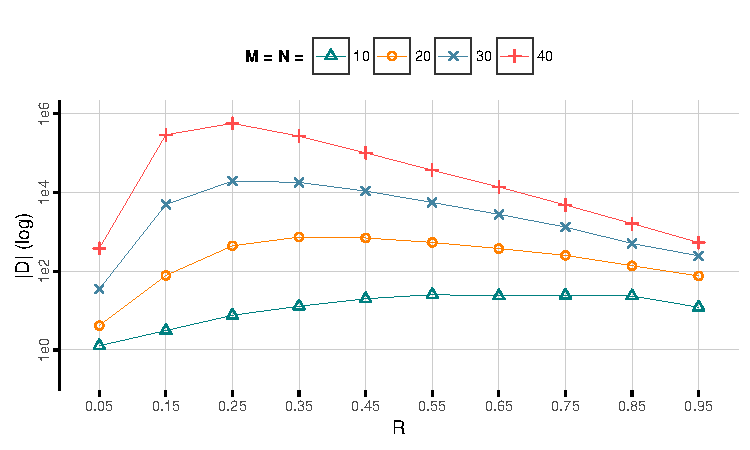
\includegraphics[trim=0em 3em 1em 0em, clip, page=1]{figures/mhs2/figures/optim_small2}
  \\[0.3em]
  \includegraphics[trim=0em 0.5em 1em 4em, clip, page=2]{figures/mhs2/figures/optim_small2}
  \caption{$(M,N,R)$ parameters' impact\label{fig:parameters-impact}}
\end{figure}
%
To better understand how the parameters affect the problem's solution,
consider the following observations (\Cref{fig:parameters-impact}):
\begin{enumerate}
\item For the same $(M,N)$ parameter values:
  \begin{enumerate}
  \item The average \ac{MHS} cardinality for problems generated with
    smaller $R$ values is larger than the average \ac{MHS} cardinality
    for problems generated with larger $R$ values (\ie, the \ac{MHS}
    cardinality is negatively correlated with the $R$ value).
  \item The average solution size (\ie, $|D|$) was minimal for
    problems generated with $R=0.05$.
  \item  $|D|$ was \textbf{not}
    maximal for problems generated with $R=0.95$.
  \end{enumerate}
\item Problems generated with larger $(M,N)$ values have the maximal
  $|D|$ value for smaller $R$ values than problems generated with
  smaller $(M,N)$ values (\ie, the value of $R$ for maximal $|D|$ is
  negatively correlated with $(M,N)$).
\end{enumerate}

\subsection{Small problems}
\label{sec:mhs2o:results:small}
The first benchmark in this section is aimed at evaluating the impact
of each optimization for small problems, for which all \acp{MHS} can
be calculated ($M = N \in \set{10, 20, 30, 40}$, and $R \in
\set{0.05,0.15,...,0.95}$).

\begin{figure}[!ht]
  \includegraphics[page=3]{figures/mhs2/figures/optim_small}
  \caption{Small problems' results\label{fig:mhs2o:results:small}}
\end{figure}

In \Cref{fig:mhs2o:results:small}, we observe the throughputs%
%
\footnote{The throughput metric is calculated as the number of
  generated \acp{MHS} divided by the total run-time and is measured in
  \acp{MHS}/sec. When calculating this metric, we took care to discard
  all non-minimal \acp{HS}.}
%
for $5$ different implementations of the algorithm with an increasing
number of features.
%
At one end of the scale, \setupName{Baseline} represents an
implementation with no optimizations as well as no heuristic (\ie,
random ranking).
%
At the other end, \Opts{1}{3} represents an implementation with both
the \setupName{Ochiai} heuristic and all the proposed optimizations
(the ids are presented in \Cref{alg:mhs2o}).
%
\setupName{Heuristic} represents the performance of \staccato{}.
%
For readability, data points for which the throughput was less than
$0.1$ \ac{MHS}/sec were omitted from the plots.




The analysis of the results shows that the heuristic by itself
introduces a significant performance improvement over
\setupName{Baseline} for $M = N = 10$ ($5\times$ faster on average,
note the log scale).
%
Such result presents a strong evidence that using a heuristic to
drive the search can not only improve the quality of the computed
\acp{MHS} (as shown in \citep{Abreu09b}) but also improve the
computational efficiency of the algorithm.
%
Additionally, and in comparison to the \setupName{Heuristic} (\ie,
\staccato{}) performance, all the optimizations showed an improved
performance of at least $1.5\times$ (\Opt{1} for $R=0.95$), at
most $170000\times$ (\Opts{1}{3} for $R=0.05$), and on average
$34000\times$, $8000\times$, and $1700\times$ for \Opts{1}{3},
\Opts{1}{2}, and \Opt{1} respectively.

Analyzing the remaining tests cases ($M = N \in \set{20,30,40}$), we
can see that, with the increase of the problem size and for small $R$
values, the relative contribution of each optimization becomes more
significant (for $M = N \in \set{10,20,30}, R=0.05$, \Opts{1}{3}
performs $30\times$, $7000\times$, and $1000000\times$ faster than
\Opt{1}, respectively).
%
We also observe that, on average and for all combinations of
$(M,N,R)$, \Opts{1}{3} was the algorithm with the best
performance, implying that the computational savings introduced by
optimization $3$ should, on average, outweigh its overhead.

It also worth understanding how each optimized implementation
improves over \setupName{Heuristic}.
%
A closer inspection of the results reveals the following patterns:
\begin{enumerate}[nolistsep,topsep=0pt]
\item All algorithms have similar performances for large $R$ values.
\item All optimizations are more effective for smaller $R$ values.
\item Optimizations $1$ and $2$ have a considerable effect for all $R$
  values whereas optimization $3$ is only effective for small $R$
  values.
\end{enumerate}
%
Pattern $1$ can be explained by noting that the average \ac{MHS}
cardinality is negatively correlated with the $R$ value.
%
It follows then that, problems with large $R$ values have shallow
search trees and, consequently, the optimizations, which focus on
improving the search tree exploration, have a lesser performance
impact.

Conversely, pattern $2$ can be explained using the complimentary
argument.
%
For small $R$ values, as the search trees become deeper, the
non-optimized algorithms perform a large amount of unnecessary divide
tasks, thus leaving (exponentially) more room for improvements.

To explain pattern 3, we shall look at the optimizations individually:
%
\begin{itemize}[nolistsep]
\item Optimization $1$ prevents the exploration of paths composed of
  the same elements although in different orders. Such inefficiencies
  occur whenever the \acp{MHS} are composed of more than $1$ element.
  %
\item Optimization $2$ reduces the overhead associated with the
  heuristic calculation. The overhead reduction also occurs whenever
  the \acp{MHS} are composed of more than $1$ element.
  %
\item Optimization $3$ performs a look-ahead verification to assess
  whether the current sub-tree is a dead-end (\ie, no \acp{MHS} will
  be generated in such sub-tree) and terminate the exploration if a
  dead end is reached. The impact of this optimization is contingent
  on how far ahead it detects the dead-end which, in turn, is
  dependent on the deepness of the search tree. As the deepness of the
  search tree is negatively correlated with $R$, this optimization is
  more effective for small $R$ values.
\end{itemize}

\subsection{Large problems}
\label{sec:mhs2o:results:large}
The second benchmark is aimed at evaluating the impact of each
optimization for large problems where it is impractical to calculate
all \acp{MHS} ($M = N = 10^3$, and $R \in \set{0.05,\cdots,0.95}$).
%
In all the following test cases a time based cutoff of $30$ seconds
was enforced.


The first two plots in \Cref{fig:mhs2o:results:large} present both the
percentage of \acp{HS} that were minimal (\ac{MHS}\%) and the average
\ac{HS} cardinality for each of the $5$ implementations.
%
For large problems, we observe that the heuristic plays an important
role in assuring that the computed \acp{HS} are in fact minimal
($98\%$ \vs{} $0\%$ minimality for \setupName{Heuristic} and
\setupName{Baseline}, on average).
%
Even though the \ac{MHS}\% of \Opts{1}{2} and \Opts{1}{3} is lower
when compared to \Opt{1}, we can see that the average \ac{HS}
cardinality of the former implementations is comparable to cardinality
of the later, implying that the number of extraneous elements in the
non-minimal \acp{HS} is small (specially when compared to
\setupName{Baseline}).

The remainder of \Cref{fig:mhs2o:results:large} presents the number of
\acp{HS} as well as the throughput for all implementations.
%
While \setupName{Baseline}, \setupName{Heuristic}, and \Opt{1} compute
$500$ \acp{HS} on average, the remaining implementations compute
$93000$ \acp{HS} on average ($186\times$ better).
%
Taking into account the number of computed \acp{HS}, despite the lower
\ac{MHS}\%, the absolute number of \acp{MHS} for optimizations $2$ and
$3$ is effectively larger than the number of \acp{MHS} calculated by
the remainder algorithms.


Finally, it is interesting to note that even though we increased the
problem size by $25\times$ factor, the throughput of \ac{MHSII} is
comparable to the throughput observed in
\Cref{fig:mhs2o:results:small}.
%
We can conclude that the fully optimized \ac{MHSII} scales to large
problems more efficiently than \staccato{}.
\begin{figure}[!ht]
  % 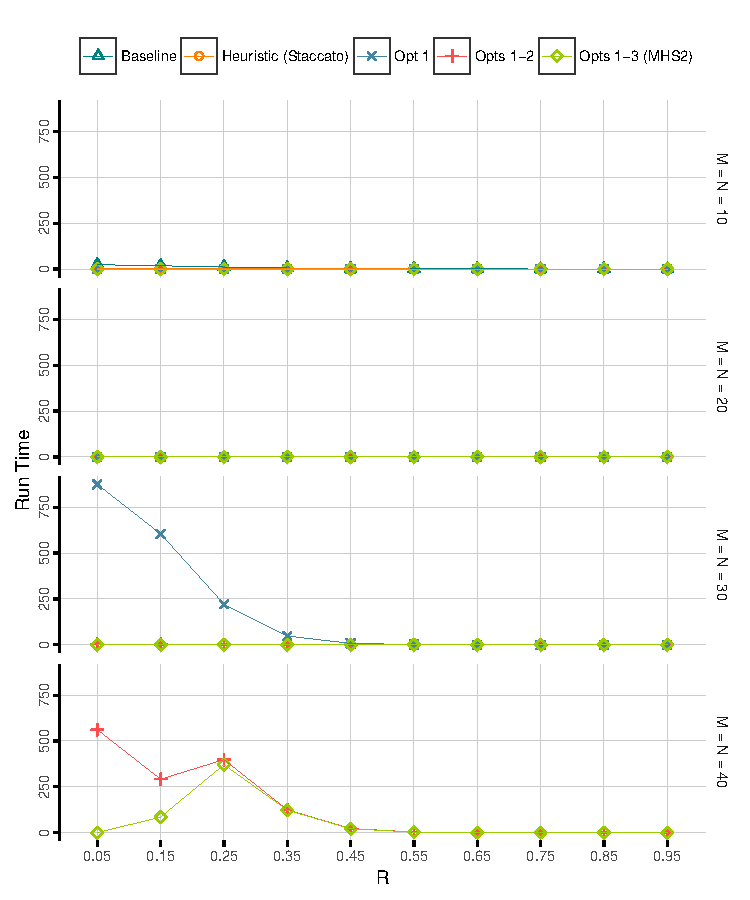
\includegraphics[trim=2em 35em 1.5em 1em, clip,
  % page=1]{figures/mhs2/figures/optim_legend}
  % \\[0.3em]
  \includegraphics[trim=0.5em 2.65em 1em 0em, clip, page=5]{figures/mhs2/figures/optim_large}
  \\[0.3em]
  \includegraphics[trim=0.5em 2.65em 1em 4em, clip, page=4]{figures/mhs2/figures/optim_large}
  \\[0.3em]
  \includegraphics[trim=0.5em 2.65em 1em 4em, clip, page=2]{figures/mhs2/figures/optim_large}
  \\[0.3em]
  % \caption{Minimality percentage/Average cardinality\label{fig:optim-large-minimal}}
  % \end{figure}
  % \begin{figure}[!ht]
  %   \ContinuedFloat
  \includegraphics[trim=0.5em 0em 1em 4em, clip, page=6]{figures/mhs2/figures/optim_large}
  \caption{Large problems' results\label{fig:mhs2o:results:large}}
  % \caption{Large problems' results (continued)\label{fig:mhs2o:results:large}}
\end{figure}


\section{Summary}
\label{sec:mhs2o:summary}
In this chapter we successfully addressed the limitations presented in
\CrefPageParen{sec:intro:research-goals:algorithmic-efficiency}
thereby positively answering \CrefPageParen{rq:optimizations}.
%
Concretely, in this chapter:
\begin{itemize}[nolistsep]
\item We proposed $3$ optimizations to \staccato{}
  (\CrefPageSee[]{sec:mhs2o:approach}):
  \begin{itemize}
  \item The first optimization prevents multiple examinations of the
    same set.
  \item The second optimization preemptively filters elements of $U$
    not contained in any set in $S$.
  \item The third optimization prevents the examination of branches
    such that there is at least one set that cannot be hit by any
    element in $U$.
  \end{itemize}
\item We provided a formal analysis of the proposed algorithm:
  \begin{itemize}
  \item We formally proved that the optimized algorithm is both sound
    and complete (\CrefPageSee[]{sec:mhs2o:analysis:soundcomplete}).
  \item We gave some intuition about the complexity of the algorithm's
    different operations
    (\CrefPageSee[]{sec:mhs2o:analysis:complexity}).
  \end{itemize}
\item We analyzed the implementation details of our reference
  implementation, which is available at \mhsIIURL{}
  (\CrefPageSee[]{sec:mhs2o:datastructures}).
\item We discussed some practical aspects of our \ac{MHS} generation
  algorithm:
  \begin{itemize}
  \item We discussed how the heuristic influences the algorithm's
    performance (\CrefPageSee[]{sec:mhs2o:heuristics}).
  \item We discussed how to improve the algorithm's performance in the
    presence of ambiguity groups
    (\CrefPageSee[]{sec:mhs2o:ambiguity-groups}).
  \item We discussed how to improve the algorithm's performance when
    solving non-minimal problems
    (\CrefPageSee[]{sec:mhs2o:problem-minimization}).
  \end{itemize}
\item We presented the conducted benchmarks showing that our
  algorithm:
  \begin{enumerate}
  \item Performs $34000\times$ faster than \staccato{} for small
    problems (\CrefPageSee[]{sec:mhs2o:results:small}).
  \item Performs $186\times$ faster than \staccato{} for large
    problems (\CrefPageSee[]{sec:mhs2o:results:large}).
  \item Exhibits a similar throughput in both small and large
    problems.
  \end{enumerate}

\end{itemize}

The faster algorithm enables the exploration of a larger number of
\ac{HS}, increasing the likelihood of actually finding the ``best''
\ac{MHS} for a particular instance of the problem.
%
In the particular case of \ac{SFL}, this improvement translates into:
\begin{itemize}[nolistsep]
\item Better diagnostic accuracy when setting a time-based cutoff,
  due to the fact that calculating more candidates increases the
  likelihood of finding the correct diagnostic candidate.
\item Smaller diagnostic latency when setting a solution size cutoff,
  due to the fact that calculating a fixed number of diagnostic
  candidates takes less time with \ac{MHSII} than with \staccato{}.
\end{itemize}
